\documentclass[]{beamer}
\mode<presentation>
{
  \usetheme{Warsaw}
  \definecolor{mcgarnet}{rgb}{0.38, 0, 0.08}
  \definecolor{mcgray}{rgb}{0.6, 0.6, 0.6}
  \setbeamercolor{structure}{fg=mcgarnet,bg=mcgray}
  %\setbeamercovered{transparent}
}


\usepackage[english]{babel}
\usepackage[latin1]{inputenc}
\usepackage{times}
\usepackage[T1]{fontenc}
\usepackage{tikz}
\usepackage{graphicx}

\newcommand{\imagesource}[1]{{\centering\hfill\break\hbox{\scriptsize Image Source:\thinspace{\small\itshape #1}}\par}}

\title{On The Foundational Crisis in Mathematics}


\author{Dr. Robert Lowe\\}

\institute[Maryville College] % (optional, but mostly needed)
{
  Division of Mathematics and Computer Science\\
  Maryville College
}

\date[]{}
\subject{}

\pgfdeclareimage[height=0.5cm]{university-logo}{images/Maryville-College}
\logo{\pgfuseimage{university-logo}}



\AtBeginSection[]
{
  \begin{frame}<beamer>{Outline}
    \tableofcontents[currentsection]
  \end{frame}
}


\begin{document}

\begin{frame}
  \titlepage
\end{frame}



% Structuring a talk is a difficult task and the following structure
% may not be suitable. Here are some rules that apply for this
% solution: 

% - Exactly two or three sections (other than the summary).
% - At *most* three subsections per section.
% - Talk about 30s to 2min per frame. So there should be between about
%   15 and 30 frames, all told.

% - A conference audience is likely to know very little of what you
%   are going to talk about. So *simplify*!
% - In a 20min talk, getting the main ideas across is hard
%   enough. Leave out details, even if it means being less precise than
%   you think necessary.
% - If you omit details that are vital to the proof/implementation,
%   just say so once. Everybody will be happy with that.

\begin{frame}{Bernhard Riemann}
\begin{columns}
    \column{0.6\textwidth}
    Georg Friedrich Bernhard Riemann
    \newline 17 September 1826 - 20 July 1866
    \begin{itemize}[<+->]
        \item Contributed to Number Theory, Analysis, and Differential
            Geometry
        \item First rigorous definition of the integral.
        \item His essay on Number Theory gave us the foundations of
            modern set theory.
        \item Wanted to make a rigorous foundation of mathematics
            grounded in set theory.
        \item His essay was the starting point for Cantor's work.
    \end{itemize}
    \column{0.4\textwidth}
    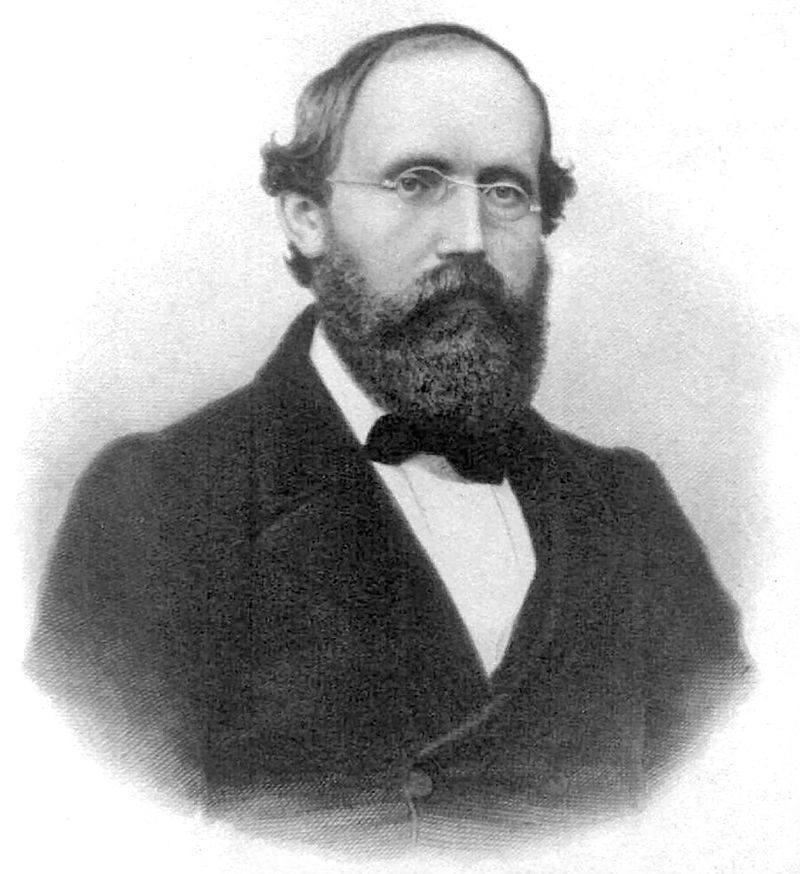
\includegraphics[width=\textwidth]{images/riemann}
    \imagesource{Wiki Commons}
\end{columns}
\end{frame}

\begin{frame}{Georg Cantor}
\begin{columns}
    \column{0.6\textwidth}
    Georg Ferdinand Ludwig Philipp Cantor
    \newline 3 March 1845 --  6 January 1918
    \begin{itemize}[<+->]
        \item Proved that the real numbers are uncountable.
        \item Proved that there is no largest cardinal number.
        \item Foundation of theory of infinite sets.
        \item Cantor's Paradox: The set of all sets is its own power
            set. Therefore the cardinal number of the set of all sets is 
            bigger than itself. (Source: Woflram Math World)
    \end{itemize}
    \column{0.4\textwidth}
    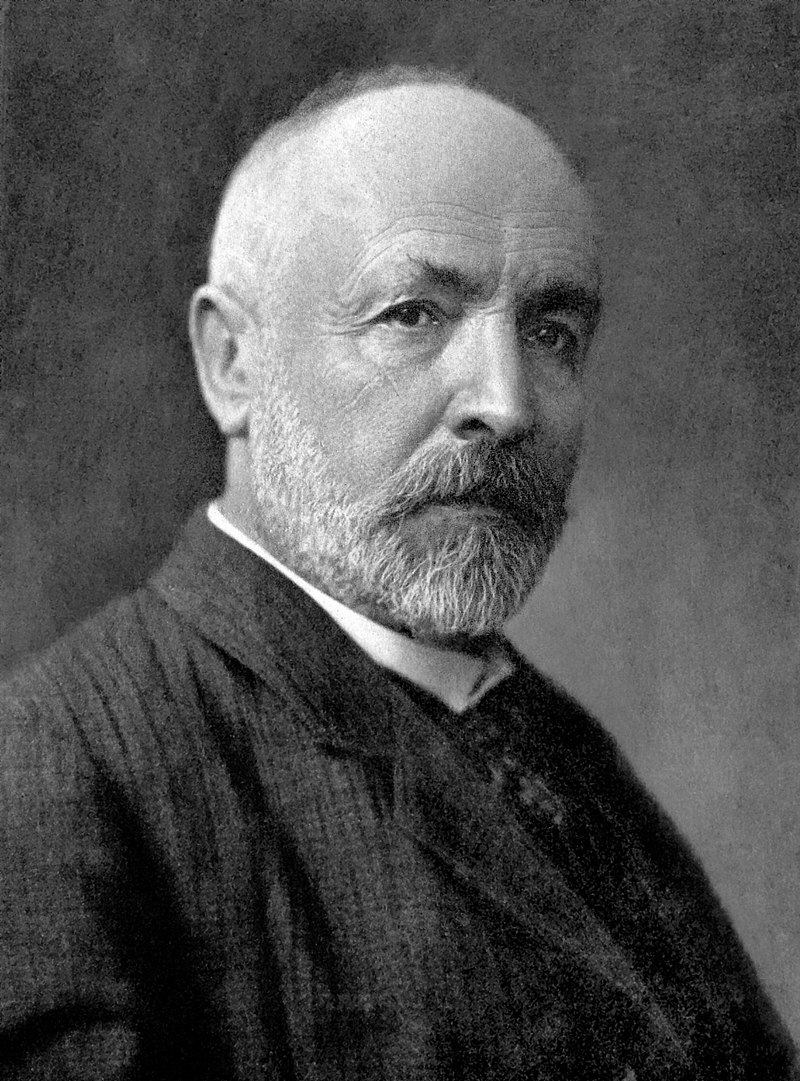
\includegraphics[width=\textwidth]{images/cantor}
    \imagesource{Wiki Commons}
\end{columns}
\end{frame}

\begin{frame}{David Hilbert}
\begin{columns}
    \column{0.6\textwidth}
    David Hilbert
    \newline 23 January 1862 -- 14 February 1943
    \begin{itemize}[<+->]
        \item One of the most influential mathematicians of the 20th
            century.
        \item Invariant theory, Calculs of Variations, Commutative
        Algebra, Algebraic Number Theory, Foundations of Geometry,
        Spectral Theory of Operators, Mathematical Physics, and Proof
        Theory
        \item Started as a logicist, later founded formalism.
    \end{itemize}
    \column{0.4\textwidth}
    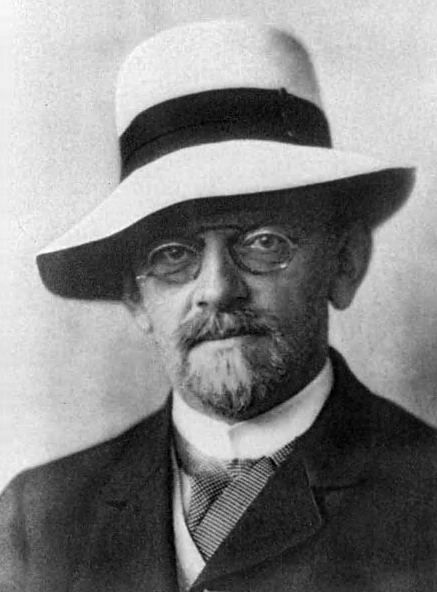
\includegraphics[width=\textwidth]{images/hilbert}
    \imagesource{Wiki Commons}
\end{columns}
\end{frame}

\begin{frame}{Luitzen Egbertus Jan Brouwer}
\begin{columns}
    \column{0.6\textwidth}
    Luitzen Egbertus Jan Brouwer
    \newline 27 February 1881 -- 2 December 1966
    \begin{itemize}[<+->]
        \item Dutch Mathematician and Philosopher
        \item Topology, Set Theory, Measure Theory, and Complex
        Analysis
        \item Founder of the Intuitionism Philosophy of Mathematics
        \item A mathematical statement corresponds to a mental
        construction, and a mathematician can assert the truth of
        a statement only by verifying the validity of that
        construction by intuition. \textit{--L.E.J. Brouwer}
    \end{itemize}
    \column{0.4\textwidth}
    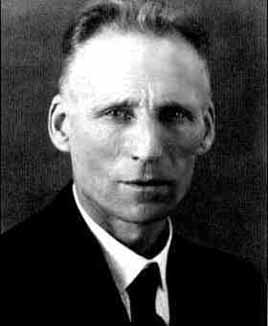
\includegraphics[width=\textwidth]{images/brouwer}
    \imagesource{Wiki Commons}
\end{columns}
\end{frame}

\begin{frame}{Bertrand Russell}
\begin{columns}
    \column{0.6\textwidth}
    Bertrand Arthur William Russell, 3rd Earl Russell
    \newline 18 May 1872 -- 2 February 1970
    \begin{itemize}[<+->]
        \item Philosopher, Mathematician, Essayist, Social Critic,
            Swell Guy
        \item Led the ``Revolt against Idealism'' in the early 20th
            century.
        \item Sparked considerable interest in formal logic through
            his works pertaining to the foundation of mathematics.
    \end{itemize}
    \column{0.4\textwidth}
    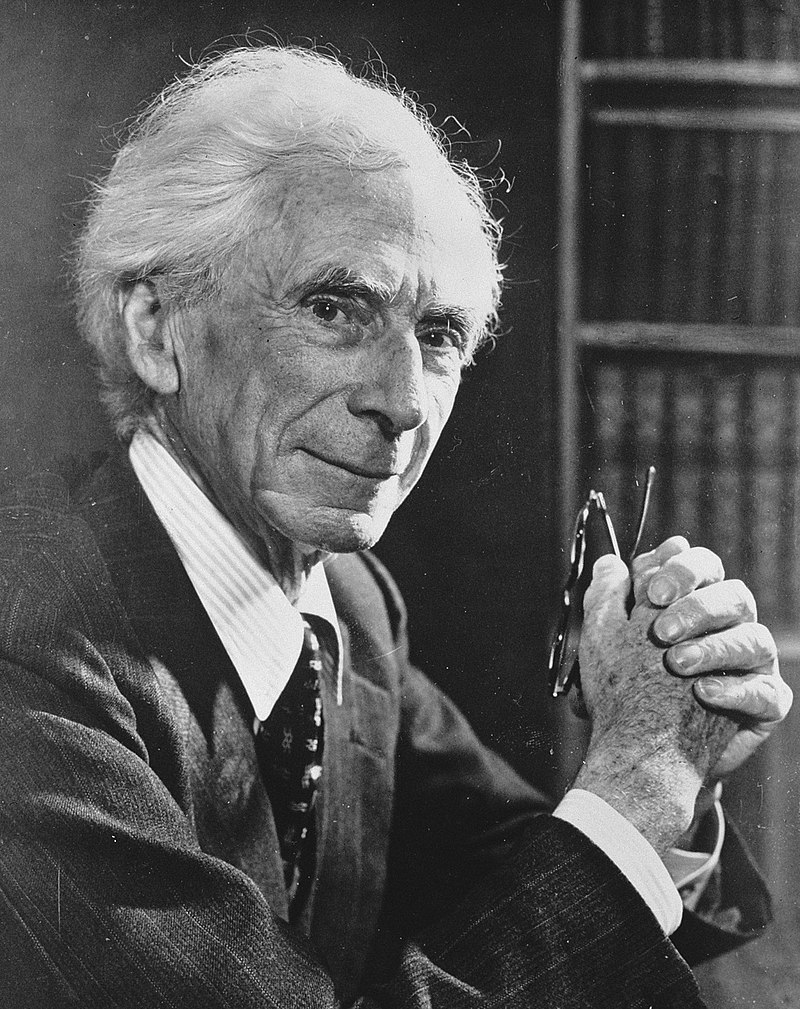
\includegraphics[width=\textwidth]{images/russell}
    \imagesource{Wiki Commons}
\end{columns}
\end{frame}

\begin{frame}{Alfred North Whitehead}
\begin{columns}
    \column{0.6\textwidth}
    Alfred North Whitehead
    \newline 15 February 1861 -- 30 December 1947
    \begin{itemize}[<+->]
        \item Mathematician and Philosopher
        \item Father of ``process philosophy''.
        \item Worked with Russell to produce \textit{Principia
        Mathematica}.
    \end{itemize}
    \column{0.4\textwidth}
    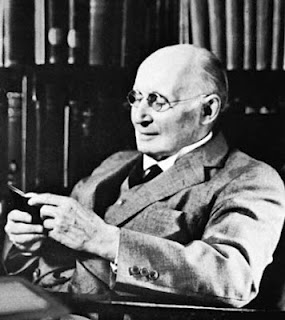
\includegraphics[width=\textwidth]{images/whitehead}
    \imagesource{Wiki Commons}
\end{columns}
\end{frame}

\begin{frame}{Kurt G\"odel}
\begin{columns}
    \column{0.6\textwidth}
    Kurt Friedrich G\"odel
    \newline 28 April 1906 -- 14 January 1978
    \begin{itemize}[<+->]
        \item Logician, Mathematician, and Analytic Philosopher
        \item A Friend of Albert Einstein
        \item Known for his Incompleteness Theorems
        \item Basically proved that Hilbert's program was not
        realizable.
    \end{itemize}
    \column{0.4\textwidth}
    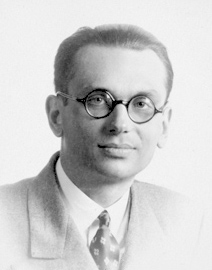
\includegraphics[width=\textwidth]{images/godel}
    \imagesource{Wiki Commons}
\end{columns}
\end{frame}

\begin{frame}{Alonzo Church}
\begin{columns}
    \column{0.6\textwidth}
    Alonzo Church
    \newline 14 June 1903 -- 11 August 1995
    \begin{itemize}
        \item Mathematician, Logician, and Computer Scientist
        \item Doctoral Advisor of Alan Turing
        \item Created $\Lambda$-Calculus which formalizes computation.
        \item Proved that the Entscheidungsproblem was undecidable.
    \end{itemize}
    \column{0.4\textwidth}
    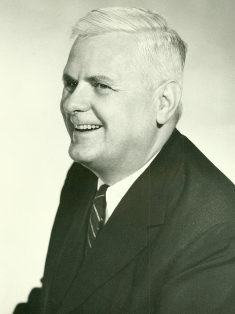
\includegraphics[width=\textwidth]{images/church}
    \imagesource{Wiki Commons}
\end{columns}
\end{frame}

\begin{frame}{Alan Turing}
\begin{columns}
    \column{0.6\textwidth}
    Alan Mathison Turing
    \newline 23 June 1912 -- 7 June 1954
    \begin{itemize}[<+->]
        \item Logician, Cryptographer, Mathematician, Father of
            Computer Science
        \item Part of the Group that broke the German enigma code.
        \item Famous for ``Turing Machines'' which formalizes
            computation and proved the undecidability of the
            Entscheidungsproblem.
    \end{itemize}
    \column{0.4\textwidth}
    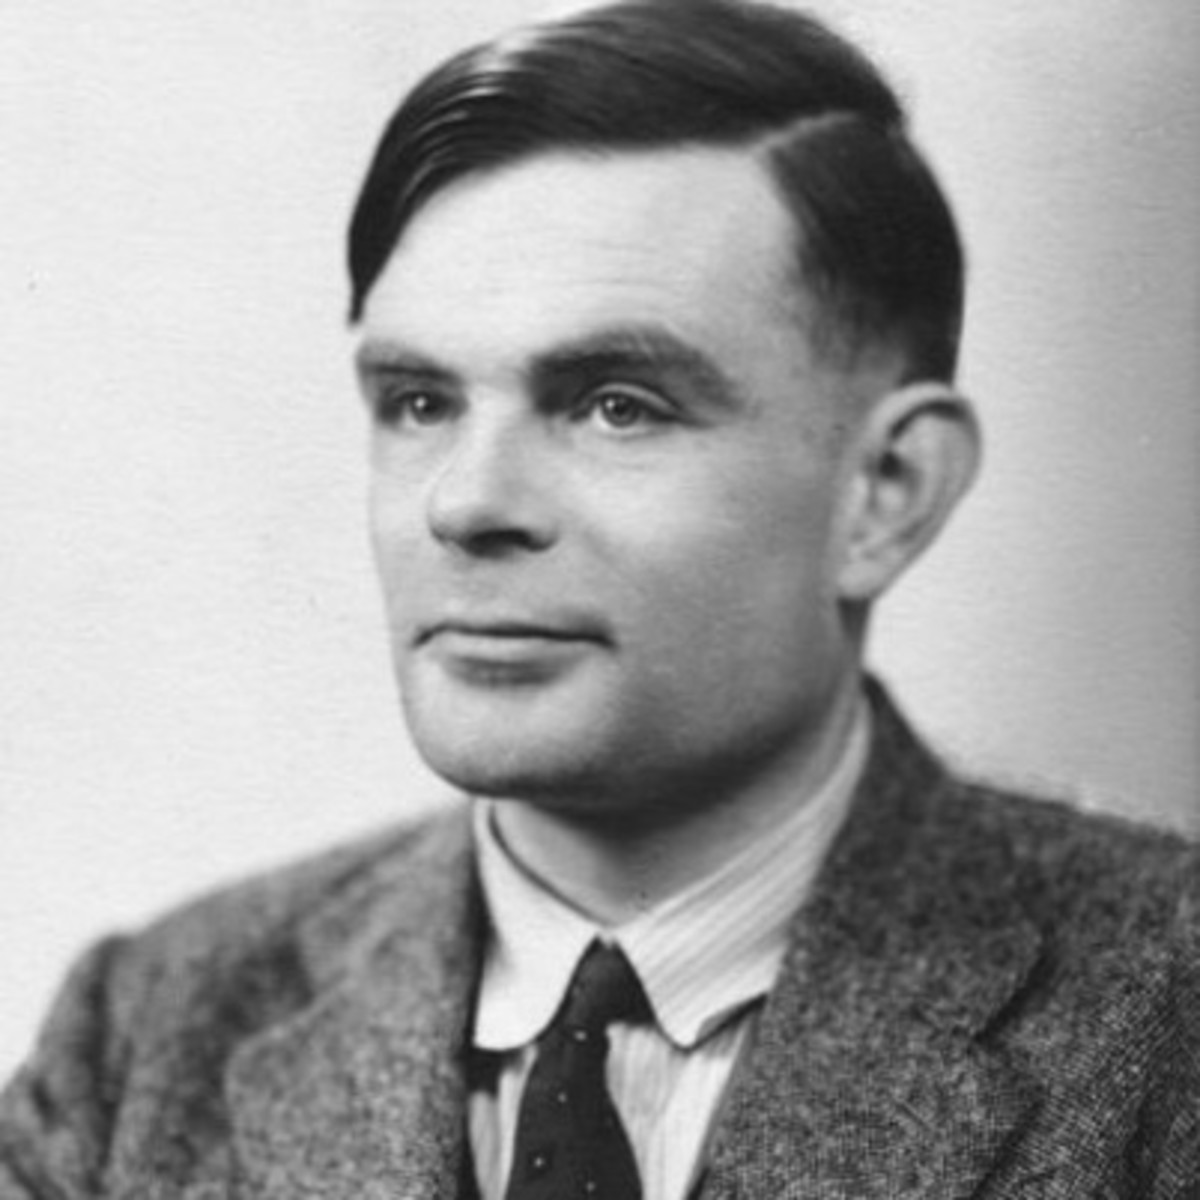
\includegraphics[width=\textwidth]{images/turing}
    \imagesource{Wiki Commons}
\end{columns}
\end{frame}


\end{document}


